\documentclass[a4paper,11pt]{beamer}
\usepackage{etex}
\usepackage{lmodern}
\usepackage[french]{babel}
\usepackage[T1]{fontenc}
\usepackage[utf8]{inputenc}
% \usepackage{listings}
\usepackage{graphicx} 
\usepackage{ragged2e}
\usepackage{enumitem}
\usepackage{array}
% \usepackage{tikz}  
% \usepackage{pgf-umlcd} 
\usepackage{csquotes}
\usepackage{pst-sigsys}
\usepackage{amsmath,amsfonts,bm}
\usepackage{pstricks-add}
% \usepackage{physics}
% \usepackage{ulem}
% \usepackage{wasysym}
\usepackage{hyperref}
% \usepackage{color}


\setenumerate{label*=\arabic*.} 

\setbeamertemplate{navigation symbols}{}  
  
\usetheme{Darmstadt} 
\setbeamertemplate{footline}{\insertframenumber/\inserttotalframenumber}
\title{L3 - CMI017 : Signaux et Systèmes\\Séquence IV}
\author{BULOUP Frank}
\institute{Aix Marseille Université\\Institut des Sciences du Mouvement}
\date{}

\setbeamertemplate{footline} 
{  
	\begin{beamercolorbox}[ht=2.5ex,dp=1.125ex,%
      leftskip=.3cm,rightskip=.3cm plus1fil]{title in head/foot}%
      {\usebeamerfont{title in head/foot}\insertshorttitle} \hfill    
      \insertframenumber / \inserttotalframenumber%
    \end{beamercolorbox}%
%     \begin{beamercolorbox}[colsep=1.5pt]{lower separation line foot}
%     \end{beamercolorbox} 
}

\newcounter{exampleBlockCounter}
\setcounter{exampleBlockCounter}{1}

\definecolor{comment}{rgb}{0.12, 0.38, 0.18 } %adjusted, in Eclipse: {0.25, 0.42, 0.30 } = #3F6A4D
\definecolor{keyword}{rgb}{0.37, 0.08, 0.25}  % #5F1441
\definecolor{string}{rgb}{0.06, 0.10, 0.98} % #101AF9
\definecolor{myGreen}{rgb}{0,0.4,0}

% \lstset {language=Java,
%  frame=single,
%  frameround=tttt,
%  rulesepcolor=\color{black},
%  showspaces=false,showtabs=false,tabsize=2,
%  numberstyle=\tiny,numbers=left,
%  stringstyle=\color{string},
%  keywordstyle = \color{keyword}\bfseries,
%  commentstyle=\color{comment}\itshape,
%  basicstyle=\ttfamily\footnotesize,
%  breaklines=true,
%  captionpos=b
% }

% \renewenvironment{package}[2][\umlcdPackageTitle]{
% \edef\umlcdPackageTitle{#2}
% \def\umlcdPackageFit{}
% \def\umlcdPackageName{#1}
% }{
%   \begin{pgfonlayer}{background}
%   \node[umlcd style, draw, inner sep=0.5cm, fit = \umlcdPackageFit] (\umlcdPackageName) {};
%   \node[umlcd style, draw, outer ysep=-0.5, anchor=south west] (\umlcdPackageName caption) at
%   (\umlcdPackageName.north west) {\umlcdPackageTitle};
%   \end{pgfonlayer}
% }

\begin{document}

\begin{frame}[plain]  
	\titlepage  
	\center{
\includegraphics[scale=0.75]{images/by-nc-sa.eps}}
	\vspace{1cm}
	
	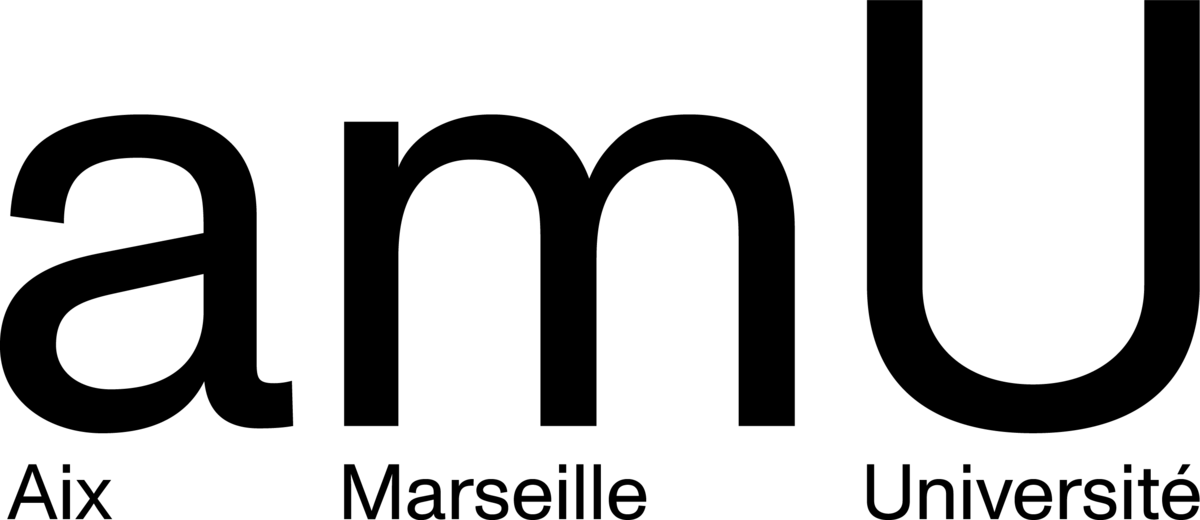
\includegraphics[scale=0.6]{images/LogoAMU.png}\hspace*{2cm}
	
\includegraphics[scale=0.2]{images/LogoCNRS.eps}\hspace*{2cm}
	
\includegraphics[scale=0.1]{images/LogoISM.eps}
\end{frame} 
  

\begin{frame}{Plan de cette séquence}
	\tableofcontents[hideallsubsections]
\end{frame}

\AtBeginSection[]{
\begin{frame}{Signaux et Systèmes}
	\tableofcontents[currentsection,hideallsubsections]
\end{frame}
}

\begin{frame}{Rappels 1/2}
\begin{alertblock}{Rappel I}
\justifying
Un SDLIT peut être définit par :
\begin{enumerate}
  \item son EAD
  \item son diagramme bloc
  \item sa fonction de transfert en $\mathcal{R}$
\end{enumerate}
\end{alertblock}
\pause
\begin{alertblock}{Rappel II}
\justifying
La réponse impulsionnelle d'un SDLIT est la réponse de ce système à une
impulsion unitaire. C'est une caractéristique fondamentale de ce dernier.
\end{alertblock}
\end{frame}

\begin{frame}{Rappels 2/2}
\begin{alertblock}{Rappel III}
\justifying
Pour les systèmes non bouclés, l'ensemble des coefficients des puissances de
$\mathcal{R}$ de la fonction de transfert donne directement la réponse impulsionnelle.
\end{alertblock}
\pause
\begin{alertblock}{Rappel IV}
\justifying
Pour les systèmes bouclés, la fonction de transfert en $\mathcal{R}$ est une
fonction rationnelle et le développement en puissance de $\mathcal{R}$ peut
être obtenu pas division polynomiale.
\end{alertblock}
\end{frame}

\section[Rép. d'un SDLIT à une entrée quelconque]{Réponse d'un SDLIT à une
entrée quelconque}
\subsection{Présentation}
\begin{frame}
\centering
\textbf{\textcolor{red}{On peut considérer tout signal numérique comme une
somme pondérée et décalée dans le temps d'impulsions unitaires}}
\vspace{1cm}

\justifying
Par exemple le signal $s(n)$ dont les valeurs successives sont 1, 2, 4, 3 puis 0
indéfiniment depuis l'origine du temps peut être exprimé de la façon suivante :
$$
s(n) = 1\cdot \delta(n) + 2\cdot \delta(n-1) + 4\cdot \delta(n-2) + 3\cdot
\delta(n-3)
$$
\end{frame}

\begin{frame}
\centering
\textbf{\textcolor{red}{De plus, on ne considère que les SDLIT}}
\vspace{1cm}

\justifying
Donc la réponse du système à $\alpha\delta(n)$ est la réponse impulsionnelle
pondérée par $\alpha$, d'après l'hypothèse de linéarité
\vspace{1cm}

\pause
Et la réponse du système à $\delta(n-n_0)$ est la réponse impulsionnelle décalée
de $n_0$, d'après l'hypothèse de stationnarité
\end{frame}

\subsection{Convolution}
\begin{frame}
\justifying
Pour obtenir la réponse d'un SDLIT à une entrée quelconque, il suffit de
développer l'entrée en somme d'impulsions unitaires pondérées et décalées
temporellement puis de sommer les réponses impulsionnelles individuelles
\vspace{0.25cm}

\pause
\centering
\begin{tabular}{p{4cm}p{4cm}}

	\psset{unit=0.5cm}
	\begin{pspicture}[showgrid=false](-1,-0.5)(5,1.5)
		\rput(-1, 1){$e(n)$}
		\rput(4.75, -0.5){$n$}
		\psaxes[labels=none]{->}(0,0)(-1,-0.5)(5,1.5)
		\psstem(-1,1){0,1,1,0,0,0,0}
		\psldots(4,0.5)
		\rput(-1, -1.25){\huge $=$}
	\end{pspicture}

&

\\
	\psset{unit=0.5cm}
	\begin{pspicture}[showgrid=false](-1,-0.5)(5,1.5)
		\rput(4.75, -0.5){$n$}
		\psaxes[labels=none]{->}(0,0)(-1,-0.5)(5,1.5)
		\psstem(-1,1){0,1,0,0,0,0,0}
		\psldots(4,0.5)
		\psline[linewidth=3pt]{->}(5.5,0)(7.5,0)
	\end{pspicture}

&
	\psset{unit=0.5cm}
	\begin{pspicture}[showgrid=false](-1,-0.5)(5,1.5)
		\rput(4.75, -0.5){$n$}
		\psaxes[labels=none]{->}(0,0)(-1,-0.5)(5,1.5)
		\psstem(-1,1){0,0.5,0.5,0,0,0,0}
		\psldots(4,0.5)
	\end{pspicture}

\\
	\psset{unit=0.5cm}
	\begin{pspicture}[showgrid=false](-1,-0.5)(5,1.5)
		\rput(4.75, -0.5){$n$}
		\psaxes[labels=none]{->}(0,0)(-1,-0.5)(5,1.5)
		\psstem(-1,1){0,0,1,0,0,0,0}
		\psldots(4,0.5)
		\rput(-1, 1.75){\huge $+$}
		\psline[linewidth=3pt]{->}(5.5,0)(7.5,0)
	\end{pspicture}

&
	\psset{unit=0.5cm}
	\begin{pspicture}[showgrid=false](-1,-0.5)(5,1.5)
		\rput(4.75, -0.5){$n$}
		\psaxes[labels=none]{->}(0,0)(-1,-0.5)(5,1.5)
		\psstem(-1,1){0,0,0.5,0.5,0,0,0}
		\psldots(4,0.5)
		\rput(-1, 1.75){\huge $+$}
		\rput(-1, -1.25){\huge $=$}
	\end{pspicture}

\\

&
	\psset{unit=0.5cm}
	\begin{pspicture}[showgrid=false](-1,-0.5)(5,1.5)
		\rput(-1, 1){$s(n)$}
		\rput(4.75, -0.5){$n$}
		\psaxes[labels=none]{->}(0,0)(-1,-0.5)(5,1.5)
		\psstem(-1,1){0,.5,1,.5,0,0,0}
		\psldots(4,0.5)
	\end{pspicture}
\\
\end{tabular}

\end{frame}

\begin{frame}
\begin{figure}
	\begin{pspicture}[showgrid=false](0,3)(11,7)
		\psset{arrows=->}

		\psfblock[framesize=1.5 0.65](5.5,6.5){h1}{Système}
		\rput(2,6.5){$\delta (n)$}
		\rput(9,6.5){$h(n)$ : rép. imp.}
		\psline{->}(4,6.5)(4.75,6.5)
		\psline{->}(6.25,6.5)(7,6.5)
		
		\pause

		\psfblock[framesize=1.5 0.65](5.5,5.5){h2}{Système}
		\rput(2,5.5){$\delta (n - k)$}
		\rput(9,5.5){$h(n - k)$}
		\psline{->}(4,5.5)(4.75,5.5)
		\psline{->}(6.25,5.5)(7,5.5)
		
		\pause
		
		\psfblock[framesize=1.5 0.65](5.5,4.5){h3}{Système}
		\rput(2,4.5){$e(k)\delta (n - k)$}
		\rput(9,4.5){$e(k)h(n - k)$}
		\psline{->}(4,4.5)(4.75,4.5)
		\psline{->}(6.25,4.5)(7,4.5)
		
		\pause
		
		\psfblock[framesize=1.5 0.65](5.5,3.5){h4}{Système}
		\rput(1.8,3.5){$
		\begin{aligned}
		e(n) = \sum_{k=0}^{+\infty} e(k)\delta (n - k)
		\end{aligned}
		$}
		\rput(9.2,3.5){$
		\begin{aligned}
		s(n) = \sum_{k=0}^{+\infty} e(k)h(n - k)
		\end{aligned}
		$}
		\psline{->}(6.25,3.5)(7,3.5)
		\psline{->}(4,3.5)(4.75,3.5)

	\end{pspicture}
\end{figure}

\end{frame}

\begin{frame}
\begin{figure}
	\begin{pspicture}[showgrid=false](0,3)(11,7)
		\psset{arrows=->}

		\psfblock[framesize=1.5 0.65](5.5,6.5){h1}{Système}
		\psfblock[framesize=1.5 0.65](5.5,5.5){h2}{Système}
		\psfblock[framesize=1.5 0.65](5.5,4.5){h3}{Système}
		\psfblock[framesize=1.5 0.65](5.5,3.5){h4}{Système}

		\rput(2,6.5){$\delta (n)$}
		\rput(2,5.5){$\delta (n - k)$}
		\rput(2,4.5){$e(k)\delta (n - k)$}
		\rput(1.8,3.5){$
		\begin{aligned}
		e(n) = \sum_{k=0}^{+\infty} e(k)\delta (n - k)
		\end{aligned}
		$}

		\rput(9,6.5){$h(n)$ : rép. imp.}
		\rput(9,5.5){$h(n - k)$}
		\rput(9,4.5){$e(k)h(n - k)$}
		\rput(9.2,3.5){$
		\begin{aligned}
		s(n) = \sum_{k=0}^{+\infty} e(k)h(n - k)
		\end{aligned}
		$}

		\psline{->}(4,6.5)(4.75,6.5)
		\psline{->}(4,5.5)(4.75,5.5)
		\psline{->}(4,4.5)(4.75,4.5)
		\psline{->}(4,3.5)(4.75,3.5)

		\psline{->}(6.25,6.5)(7,6.5)
		\psline{->}(6.25,5.5)(7,5.5)
		\psline{->}(6.25,4.5)(7,4.5)
		\psline{->}(6.25,3.5)(7,3.5)

	\end{pspicture}
\end{figure}
\justifying 
Les hypothèses de linéarité et d'invariance temporelle permettent d'obtenir une
relation entrée/sortie générique : la sortie d'un système LIT discret est une
somme pondérée de réponses impulsionnelles renversées et décalées
temporellement.\\
\vspace{0.25cm}

\centering
C'est la \textbf{\textcolor{red}{convolution}}
\end{frame}

\begin{frame}
\centering
\textbf{
\textcolor{red}{
On a : 
$$
\mathcal{H}(\mathcal{R}) = \sum_{k=0}^{+\infty}h(k)\mathcal{R}^k
$$
$h(k)$ étant la réponse impulsionnelle du système. On peut obtenir la sortie du
système à une entrée quelconque en utilisant la relation de
convolution :
$$
s(n) = \sum_{k=0}^{+\infty} e(k)h(n - k)
$$
}}
\end{frame}

\section[La TZ]{La Transformée en z} 
\subsection{Généralités}    

\begin{frame}
\begin{block}{Définition}
Soit $x(n)$ un signal discret. La transformée en z de $x(n)$ est définie par :
$$
X(z) = \sum_{n=0}^{+\infty}x(n)z^{-n}
$$
\end{block}
\pause
\begin{exampleblock}{Exercice \Roman{exampleBlockCounter} - Calculs de TZ}
Calculer les transformées en z des signaux suivants :
\begin{enumerate}
  \item $\delta (n)$
  \item $\delta (n-1)$
  \item $x_1(n) = (\frac{1}{4})^n$
  \item $x_2(n)=\alpha^n$
\end{enumerate}
\end{exampleblock}
\end{frame}

\begin{frame}
\begin{exampleblock}{Exercice \Roman{exampleBlockCounter} - Calculs de TZ}
$$
\begin{aligned}
X_2(z) &= \sum_{n=0}^{+\infty}\alpha^n \cdot z^{-n}\\
\pause
&= \sum_{n=0}^{+\infty}(\alpha \cdot z^{-1})^{n}\\
\pause
&= \lim_{n \rightarrow +\infty} \frac{1-(\alpha \cdot z^{-1})^{n+1}}{1-\alpha
\cdot z^{-1}}\\
\end{aligned}
$$
\pause
\justifying
Cette dernière expression converge si $\lvert \alpha \cdot z^{-1} \rvert<1
\Leftrightarrow \lvert z \rvert > \lvert \alpha \rvert$. Dans ce cas :
$$
X_2(z) = \frac{1}{1-\alpha z^{-1}}
$$
\end{exampleblock}
\end{frame}
\stepcounter{exampleBlockCounter}

\subsection{Lien avec la foncion de transfert en $\mathcal{R}$}
\begin{frame}
\justifying
On a vu (séquence II - slide \no$23$) que les coefficients du développement
polynomial de la fonction de transfert en $\mathcal{R}$ donnent la réponse
impulsionnelle du système :
$$
\mathcal{H}(\mathcal{R}) = \sum_{n=0}^{+\infty} h(n) \cdot \mathcal{R}^{n}
$$
Pour obtenir la fct. de trsf. en z, il suffit de remplacer $\mathcal{R}$
par $z^{-1}$ :
$$
\begin{aligned}
\mathcal{H}(z) &= \sum_{n=0}^{+\infty} h(n) \cdot z^{-n}\\
\text{ avec }\\
\mathcal{H}(z) &= \frac{S(z)}{E(z)}
\end{aligned}
$$
\pause
\centering
\textbf{
\textcolor{red}{La TZ de la réponse impulsionnelle d'un système\\
est sa fonction de transfert en z} }
\end{frame} 

\section[Obtention de la Rép. Imp.]{Obtention de la Réponse Impulsionnelle}  
\subsection{Pourquoi et comment ?}
\begin{frame}
\begin{exampleblock}{?` Question ?}
\centering
Pourquoi s'intéresser de si près à la réponse impulsionnelle ?
\end{exampleblock}
\pause
\centering
\textcolor{red}{\textbf{Parce que si l'on connait la Rep. Imp. d'un SDLIT, on
connaitra sa réponse pour toute entrée !}}
\pause
\begin{exampleblock}{?` Question ?}
\centering
Comment connaitre la réponse d'un SDLIT à une entrée quelconque ?
\end{exampleblock}
\pause
\centering
\textcolor{red}{\textbf{En utilisant la convolution !}}
\end{frame}

\subsection{En pratique}
\begin{frame}
\justifying
Il existe plusieurs méthodes d'obtention de la réponse impulsionnelle à partir
de la fonction de transfert en z. Nous utiliserons la méthode de la division
polynomiale.
\begin{exampleblock}{Exercice \Roman{exampleBlockCounter} - Calculs de Réponses
Impulsionnelles} 
\justifying
Pour chacun des systèmes caractérisés par les fonctions de
transfert en z suivantes :
$$
\begin{aligned}
\mathcal{H}_1(z) &= \frac{1}{1-\frac{1}{2}z^{-1}}\\
\mathcal{H}_2(z) &= \frac{1}{1+2z^{-1}}\\
\end{aligned}
$$
\end{exampleblock}
\end{frame}

\begin{frame}
\begin{exampleblock}{Exercice \Roman{exampleBlockCounter} - Calculs de Réponses
Impulsionnelles}
\begin{enumerate}
  \justifying
  \item Donner les valeurs des pôles de la fonction rationnelle
  \item Donner l'expression de la réponse impulsionnelle. Vérifier avec
  \textbf{impz}.
  \item La réponse impulsionnelle converge-t-elle vers zéro pour $n$ grand ?
  Concluez quant au comportement de la sortie du système à une entrée bornée.
  \item En utilisant la fonction Matlab \textbf{conv}, donner la réponse du
  système à une sinusoïde de fréquence 1Hz, échantillonnée à 1000Hz pendant
  50ms.
\end{enumerate}
\end{exampleblock}
\end{frame}
\stepcounter{exampleBlockCounter}

\begin{frame} 
\begin{alertblock}{Remarques}
\begin{enumerate}
  \item Les pôles peuvent être complexes
  \item Si des pôles ont des modules supérieurs à un, le système est instable
  \item
  \href{https://en.wikipedia.org/wiki/BIBO_stability}{\underline{Cf. stabilité
  BIBO}}
\end{enumerate}
\end{alertblock}
\end{frame}

\section[Fct. de trsf. en z]{Fonction de transfert en z}
\subsection{Propriétés de la TZ}
\begin{frame}
\begin{block}{Théorème du retard}
\justifying
Si $x(n)$ et $X(z)$ sont des paires de transformées. Alors la transformée de :
$$
y(n)=x(n-m)
$$
est :
$$
Y(z) = z^{-m}X(z)
$$
\end{block}
\end{frame}

\begin{frame}
\justifying
Soient $x(n)$ et $X(z)$ une paire de transformées. Quelle est la transformée de
$y(n)=x(n-m)$ ?
$$
\begin{aligned}
Y(z) &= \sum_{n=0}^{+\infty}x(n-m)\cdot z^{-n}
\end{aligned}
$$
\pause
Posons $k=n-m$, alors :
$$
\begin{aligned}
Y(z) &= \sum_{k=-m}^{+\infty}x(k)\cdot z^{-k-m}\\
	 &= z^{-m}\sum_{k=-m}^{+\infty}x(k)\cdot z^{-k}\\
\pause
	 &= z^{-m}\sum_{k=0}^{+\infty}x(k)\cdot z^{-k}
\end{aligned}
$$
car $x(k)=0$ si $k<0$. Finalement :
\pause
$$
\begin{aligned}
Y(z) &= z^{-m}X(z)
\end{aligned}
$$
\end{frame}

\begin{frame}
\begin{block}{Linéarité}
\justifying 
Si $x_1(n)$, $X_1(z)$ et $x_2(n)$, $X_2(z)$ sont des paires de transformées.
Alors la transformée en z de :
$$
y(n)=\alpha x_1(n) + \beta x_2(n)
$$
est :
$$
Y(z)= \alpha X_1(Z) + \beta X_2(z)
$$
\end{block}
\end{frame}

\begin{frame}
\justifying
Soient $x_1(n)$, $X_1(z)$ et $x_2(n)$, $X_2(z)$ deux paires de transformées.
Quelle est la transformée de $y(n)=\alpha x_1(n) + \beta y_1(n)$ ?
$$
\begin{aligned}
Y(z) &= \sum_{n=0}^{+\infty}[\alpha x_1(n) + \beta x_2(n)]\cdot z^{-n}\\
\pause
     &= \sum_{n=0}^{+\infty}\alpha x_1(n)\cdot z^{-n} +
        \sum_{n=0}^{+\infty}\beta x_2(n)\cdot z^{-n}\\
\pause
     &= \alpha\sum_{n=0}^{+\infty} x_1(n)\cdot z^{-n} +
        \beta\sum_{n=0}^{+\infty} x_2(n)\cdot z^{-n}\\
\pause
     &= \alpha X_1(z) + \beta X_2(z)
\end{aligned}
$$
\end{frame}

\subsection{Forme générale de la fonction de transfert en z}
\begin{frame}
\justifying
À partir de la forme générale de l'EAD :
$$
s(n) = \sum_{k=0}^{N-1}b(k)e(n-k) - \sum_{k=1}^{M-1}a(k)s(n-k)
$$
et des deux résultats précédents, il est possible d'en déduire la forme générale
de la fonction de transfert $\mathcal{H}(z)$ :
$$
\boxed{
\mathcal{H}(z) = \frac{\sum\limits_{k=0}^{N-1}b(k)\cdot
z^{-k}}{1+\sum\limits_{k=1}^{M-1}a(k)\cdot z^{-k}}
}
$$
\end{frame} 
 
\begin{frame}
\justifying
Que l'on peut réécrire de la façon suivante :
$$
\begin{aligned}
\mathcal{H}(z) &= \frac{b(0) + b(1)z^{-1} + b(2)z^{-2} + \ldots +
b(N-1)z^{-N+1}}{1 + a(1)z^{-1} + a(2)z^{-2} + \ldots + a(M-1)z^{-M+1}}\\
&= z^{M-N}b(0)\cdot \frac{(z-z_0)(z-z_1)(z-z_2)\ldots
(z-z_{N-1})}{(z-p_0)(z-p_1)(z-p_2)\ldots (z-p_{M-1})}
\end{aligned}
$$
\pause
\begin{alertblock}{Remarques}
\begin{enumerate}
  \justifying
  \item Les $z_i$ sont les zéros de $\mathcal{H}(z)$
  \item Les $p_i$ sont les pôles de $\mathcal{H}(z)$
  \item Le système est stable si tous les pôles ont des modules inférieurs à un
\end{enumerate}
\end{alertblock}
\end{frame}
 
\section{Home work !}  
\begin{frame}
\begin{exampleblock}{Exercice \Roman{exampleBlockCounter} - Calculs de Réponses
Impulsionnelles} 
\justifying
Pour les systèmes caractérisés par les fonctions de transfert
en z suivantes :
$$
\begin{aligned}
\mathcal{H}_3(z) &= \frac{1}{3} + \frac{2}{3}z^{-1} + \frac{1}{3}z^{-2}\\
\mathcal{H}_4(z) &= \frac{1}{1+z^{-1}}\\
\mathcal{H}_5(z) &= \frac{1}{(1-\frac{1}{2}z^{-1})(1+2z^{-1})}
\end{aligned}
$$
\end{exampleblock}
\end{frame}

\begin{frame}
\begin{exampleblock}{Exercice \Roman{exampleBlockCounter} - Calculs de Réponses
Impulsionnelles}
\begin{enumerate}
  \justifying
  \item Donner les valeurs des pôles de la fonction rationnelle
  \item Donner l'expression de la réponse impulsionnelle
  \item La réponse impulsionnelle converge-t-elle vers zéro pour $n$ grand ?
  Concluez quant au comportement de la sortie du système à une entrée bornée 
\end{enumerate}
\end{exampleblock}
\end{frame}
\stepcounter{exampleBlockCounter}



\end{document}
